\chapter{Pembuatan Model Termal Satelit LAPAN-A3}

Bab ini akan membahas langkah-langkah untuk membuat model termal semi-empiris
satelit LAPAN-A3 menggunakan metode \textit{machine learning}. Diagram alir
proses pembuatan model termal tersebut dapat dilihat kembali pada Gambar
\ref{fig:metodologi} yang memuat metodologi penelitan pada karya tulis ini
secara umum. Kemudian, karena persamaan-persamaan terkait perhitungan variabel
model termal sudah dibahas secara menyeluruh pada bab Tinjauan Pustaka, bab ini
hanya akan membahas bagaimana variabel pada persamaan-persamaan tersebut dapat
dihitung dari data yang sudah dikumpulkan. Penjabaran fungsi dan algoritma
dalam pembuatan model termal lebih mendalam dapat dilihat di kode sumber
pemrograman karya tulis ini yang tersedia di repositori
https://github.com/sutricky/a3thermalmodel pada situs \textit{Github}.

\section{Penyelesaian Persamaan Termal Satelit LAPAN-A3 Secara Semi-empiris}

Sesuai dengan penjelasan pada bab Tinjauan Pustaka, persamaan termal satelit
LAPAN-A3 akan diselesaikan secara semi-empiris lewat regresi linear menggunakan
metode \textit{machine learning}. Artinya, persamaan laju perubahan suhu
\textit{node} satelit yang dapat dilihat pada Persamaan \ref{eq:lineq} akan
diselesaikan dengan kombinasi data empiris serta observasi satelit dengan hasil
perhitungan koefisien persamaan tersebut lewat regresi linear yang menggunakan
modul \textit{machine learning} dalam bahasa pemrograman Python. Hanya variabel
yang tidak tersedia dari data telemetri satelit maupun dihasilkan model regresi
linear yang perlu dihitung terpisah. 

Tabel \ref{table:variabellist} merangkum sumber nilai variabel-variabel pada
Persamaan \ref{eq:lineq}. Berangkat dari variabel-variabel yang didapatkan dari
data telemetri satelit serta variabel yang masih perlu dihitung di Tabel
\ref{table:variabellist}, selanjutnya dilakukan pengumpulan data satelit terkait.

\begin{table}[!ht]
\begin{center}
	\caption{Detail sumber nilai variabel-variabel Persamaan \ref{eq:lineq}}
\label{table:variabellist}
\begin{tabular}{|l|l|l|}
\hline
Data telemetri satelit & Perhitungan & Model regresi linear                  \\ \hline
$\Delta T_{i}$         & $F_{e,i}$   & $\frac{c_S}{C_iI_0}$                  \\ \hline
$\Delta t$             & $F_{i,E}$   & $\frac{c_a}{C_i}$                     \\ \hline
$I_i$                  & $F_{a}$     & $\frac{c_E}{C_i}$                     \\ \hline
$T_i$                  &             & $\frac{\sigma R_{ij} + c_{env}}{C_i}$ \\ \hline
$T_j$                  &             & $\frac{G_{ij}}{C_i}$                  \\ \hline
$T_i^4$             &             & $\frac{\sigma R_{ij}}{C_i}$           \\ \hline
$T_j^4$             &             & $\frac{\dot{Q_{dis,i}}}{C_i}$         \\ \hline
\end{tabular}
\end{center}
\vspace{-5mm}
\end{table}

Dapat dilihat dari Tabel \ref{table:variabellist} bahwa hanya tersisa 3
variabel yang perlu dihitung : faktor gerhana \textit{node} $F_{e,i}$,
\textit{view factor node} ke Bumi $F_{i,E}$, dan faktor albedo satelit $F_{a}$. Ketiga
variabel tersebut dibutuhkan untuk menghitung faktor-faktor termal satelit yang
sudah dicantumkan pada Tabel \ref{table:unknown}. Karena itu, perhitungan ketiga variabel tersebut akan dilakukan pada bagian Perhitungan Faktor Termal Satelit.

\section{Pengumpulan Data}

Data yang diperlukan untuk penelitian di karya tulis ini dapat dibagi menjadi 2 jenis : data
telemetri satelit LAPAN-A3 serta data \textit{two-line element} (TLE). Data
telemetri satelit LAPAN-A3 diperoleh dari data operasional internal LAPAN,
sedangkan data TLE LAPAN-A3 diambil dari situs Celestrak \cite{kelso}. Kedua
jenis data dikumpulkan untuk periode observasi 19 sampai dengan 20 Mei 2018.

Data telemetri satelit LAPAN-A3 yang dibutuhkan mencakup pembacaan sensor suhu
dan sinar Matahari \textit{node-node} satelit serta sikap satelit selama
periode observasi. Sesuai dengan model satelit LAPAN-A3 yang digunakan, data
yang disediakan oleh LAPAN juga sudah berupa bacaan sensor dari 6 sisi satelit
dan plat tengah satelit. Untuk membantu visualisasi data, modul Matplotlib
digunakan sehingga didapatkan grafik-grafik representasi data telemetri satelit
LAPAN-A3 yang dikumpulkan pada 19 dan 20 Mei 2018.

Grafik suhu \textit{node-node} satelit vs waktu pada kedua periode observasi
dapat dilihat pada Gambar \ref{fig:rawtemp1219} sampai dengan
\ref{fig:rawtemp720}. Setiap titik pada grafik-grafik tersebut mewakili 1 poin
observasi pengambilan bacaan sensor pada satelit LAPAN-A3 seiring perubahan
waktu. Terdapat selang waktu antar pembacaan sensor sehingga grafik nilai
variabel terhadap waktu yang dihasilkan bersifat diskrit.

\begin{figure}[H]
\setlength\belowcaptionskip{-0.7\baselineskip}
\begin{center}
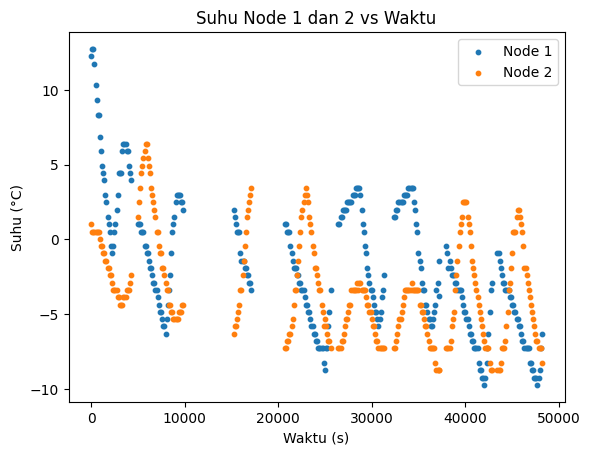
\includegraphics[width=0.7\textwidth]{fig/raw_node12_temp_2018-05-19.png}
	\caption{Grafik suhu \textit{node} 1 dan 2 satelit vs waktu pada 19 Mei 2018}
\label{fig:rawtemp1219}
\end{center}
\end{figure}

\begin{figure}[H]
\setlength\belowcaptionskip{-0.7\baselineskip}
\begin{center}
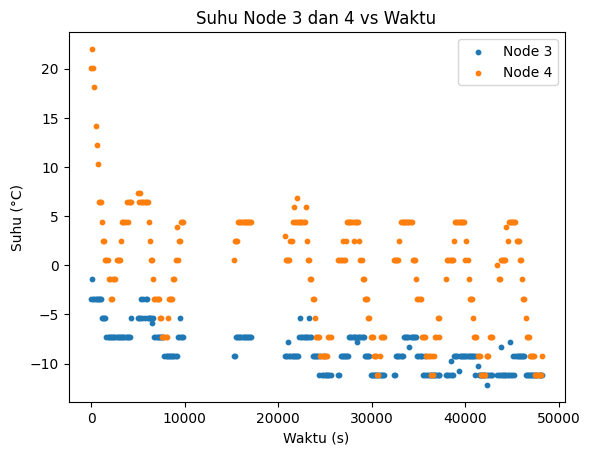
\includegraphics[width=0.7\textwidth]{fig/raw_node34_temp_2018-05-19.png}
	\caption{Grafik suhu \textit{node} 3 dan 4 satelit vs waktu pada 19 Mei 2018}
\label{fig:rawtemp3419}
\end{center}
\end{figure}

\begin{figure}[H]
\setlength\belowcaptionskip{-0.7\baselineskip}
\begin{center}
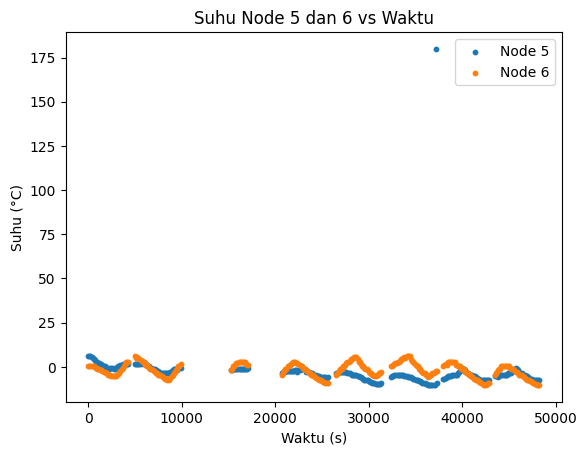
\includegraphics[width=0.7\textwidth]{fig/raw_node56_temp_2018-05-19.png}
	\caption{Grafik suhu \textit{node} 5 dan 6 satelit vs waktu pada 19 Mei 2018}
\label{fig:rawtemp5619}
\end{center}
\end{figure}

\begin{figure}[H]
\setlength\belowcaptionskip{-0.7\baselineskip}
\begin{center}
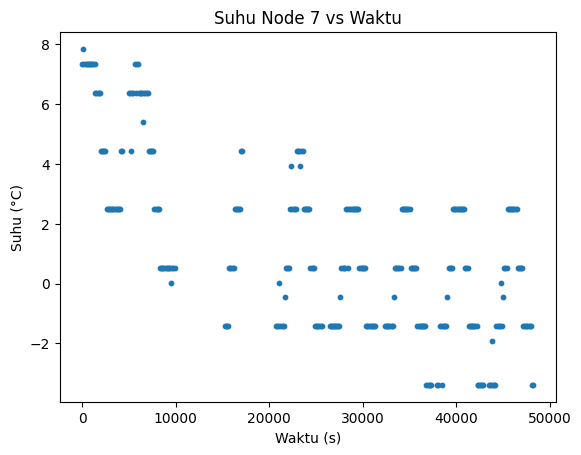
\includegraphics[width=0.7\textwidth]{fig/raw_node7_temp_2018-05-19.png}
	\caption{Grafik suhu \textit{node} 7 satelit vs waktu pada 19 Mei 2018}
\label{fig:rawtemp719}
\end{center}
\end{figure}

\begin{figure}[H]
\setlength\belowcaptionskip{-0.7\baselineskip}
\begin{center}
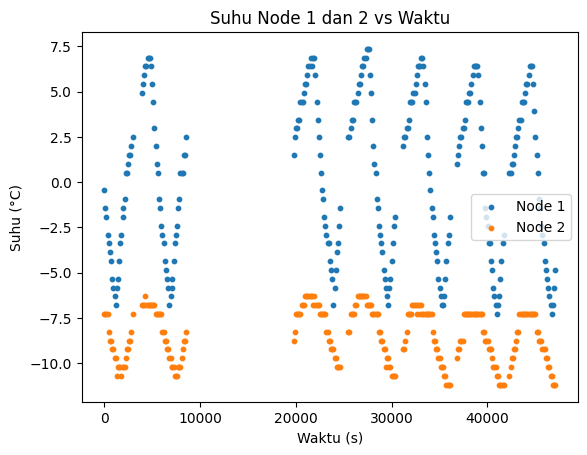
\includegraphics[width=0.7\textwidth]{fig/raw_node12_temp_2018-05-20.png}
	\caption{Grafik suhu \textit{node} 1 dan 2 satelit vs waktu pada 20 Mei 2018}
\label{fig:rawtemp1220}
\end{center}
\end{figure}

\begin{figure}[H]
\setlength\belowcaptionskip{-0.7\baselineskip}
\begin{center}
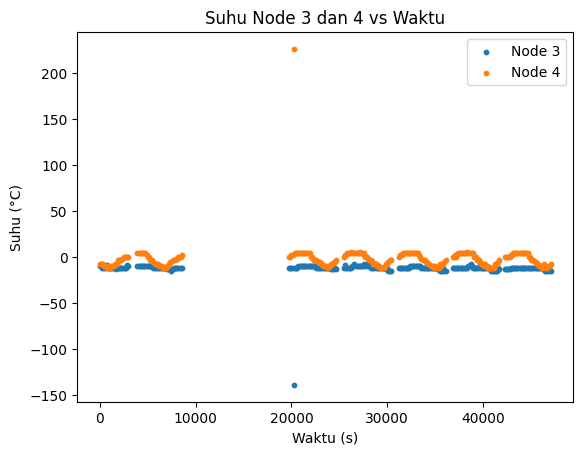
\includegraphics[width=0.7\textwidth]{fig/raw_node34_temp_2018-05-20.png}
	\caption{Grafik suhu \textit{node} 3 dan 4 satelit vs waktu pada 20 Mei 2018}
\label{fig:rawtemp3420}
\end{center}
\end{figure}

\begin{figure}[H]
\setlength\belowcaptionskip{-0.7\baselineskip}
\begin{center}
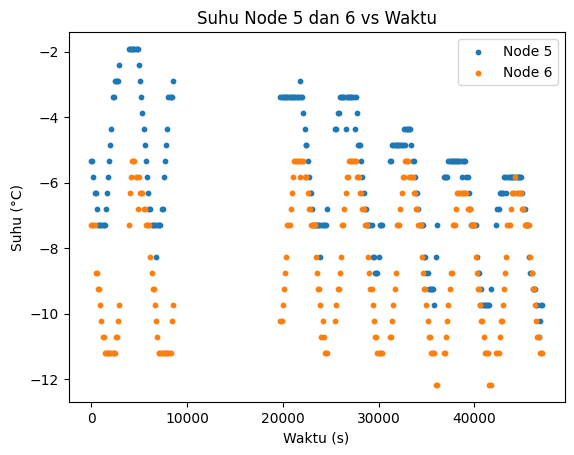
\includegraphics[width=0.7\textwidth]{fig/raw_node56_temp_2018-05-20.png}
	\caption{Grafik suhu \textit{node} 5 dan 6 satelit vs waktu pada 20 Mei 2018}
\label{fig:rawtemp5620}
\end{center}
\end{figure}

\begin{figure}[H]
\setlength\belowcaptionskip{-0.7\baselineskip}
\begin{center}
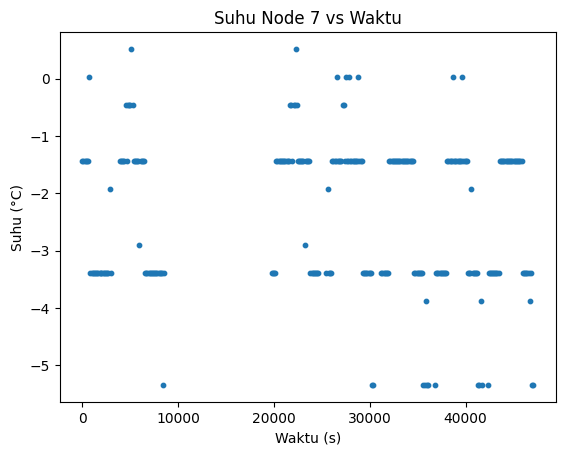
\includegraphics[width=0.7\textwidth]{fig/raw_node7_temp_2018-05-20.png}
	\caption{Grafik suhu \textit{node} 7 satelit vs waktu pada 20 Mei 2018}
\label{fig:rawtemp720}
\end{center}
\end{figure}

Berbeda dengan sensor suhu, sensor sinar Matahari pada satelit LAPAN-A3 hanya
terletak pada struktur sisi-sisi satelit. Karena \textit{node} 7 mewakili plat
tengah satelit, tidak ada sensor Matahari pada \textit{node} tersebut. Grafik
bacaan arus sensor Matahari pada \textit{node} 1 sampai dengan 6 untuk kedua
periode observasi dapat dilihat pada Gambar \ref{fig:rawcss1219} sampai dengan
\ref{fig:rawcss5620}.

\begin{figure}[H]
\setlength\belowcaptionskip{-0.7\baselineskip}
\begin{center}
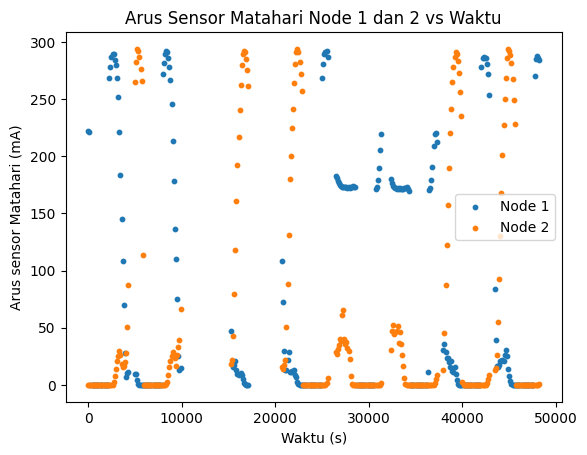
\includegraphics[width=0.7\textwidth]{fig/raw_node12_css_2018-05-19.png}
	\caption{Grafik arus sensor Matahari \textit{node} 1 dan 2 satelit vs waktu pada 19 Mei 2018}
\label{fig:rawcss1219}
\end{center}
\end{figure}

\begin{figure}[H]
\setlength\belowcaptionskip{-0.7\baselineskip}
\begin{center}
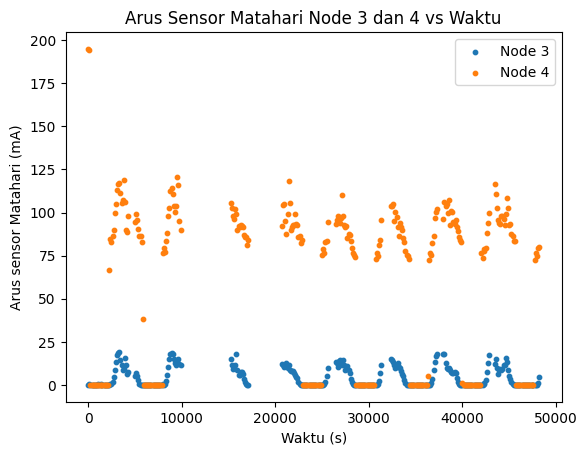
\includegraphics[width=0.7\textwidth]{fig/raw_node34_css_2018-05-19.png}
	\caption{Grafik arus sensor Matahari \textit{node} 3 dan 4 satelit vs waktu pada 19 Mei 2018}
\label{fig:rawcss3419}
\end{center}
\end{figure}

\begin{figure}[H]
\setlength\belowcaptionskip{-0.7\baselineskip}
\begin{center}
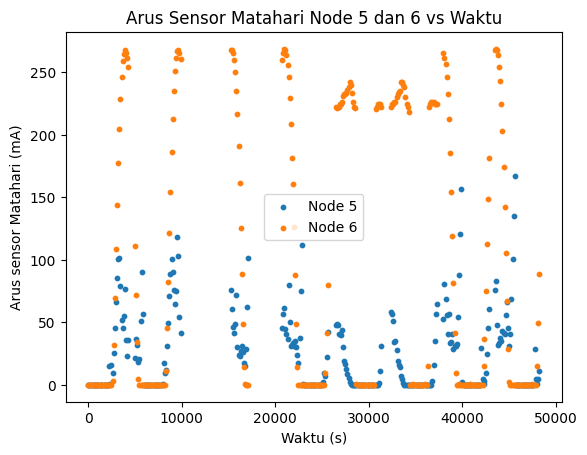
\includegraphics[width=0.7\textwidth]{fig/raw_node56_css_2018-05-19.png}
	\caption{Grafik arus sensor Matahari \textit{node} 5 dan 6 satelit vs waktu pada 19 Mei 2018}
\label{fig:rawcss5619}
\end{center}
\end{figure}

\begin{figure}[H]
\setlength\belowcaptionskip{-0.7\baselineskip}
\begin{center}
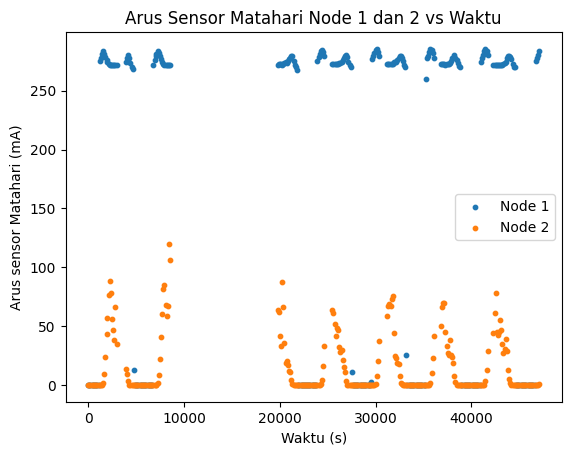
\includegraphics[width=0.7\textwidth]{fig/raw_node12_css_2018-05-20.png}
	\caption{Grafik arus sensor Matahari \textit{node} 1 dan 2 satelit vs waktu pada 20 Mei 2018}
\label{fig:rawcss1220}
\end{center}
\end{figure}

\begin{figure}[H]
\setlength\belowcaptionskip{-0.7\baselineskip}
\begin{center}
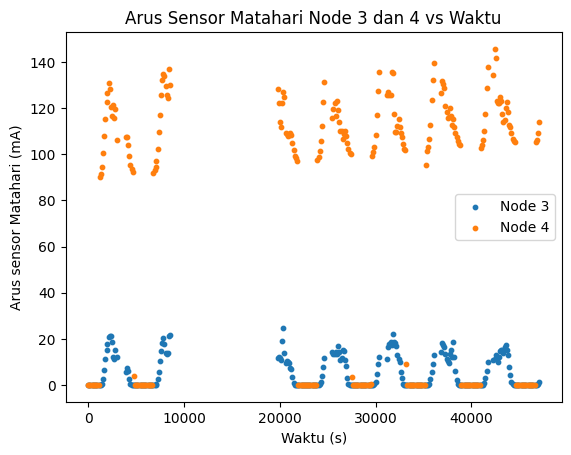
\includegraphics[width=0.7\textwidth]{fig/raw_node34_css_2018-05-20.png}
	\caption{Grafik arus sensor Matahari \textit{node} 3 dan 4 satelit vs waktu pada 20 Mei 2018}
\label{fig:rawcss3420}
\end{center}
\end{figure}

\begin{figure}[H]
\setlength\belowcaptionskip{-0.7\baselineskip}
\begin{center}
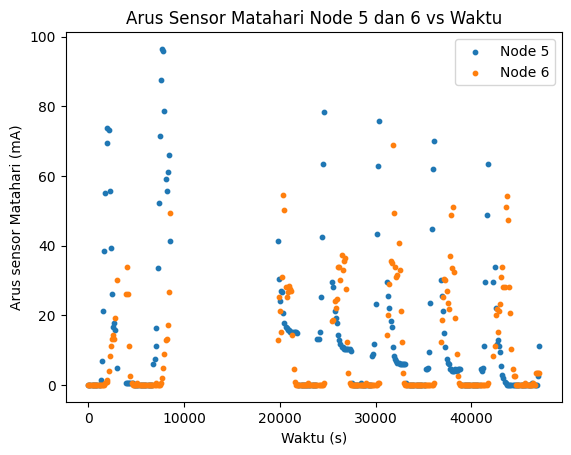
\includegraphics[width=0.7\textwidth]{fig/raw_node56_css_2018-05-20.png}
	\caption{Grafik arus sensor Matahari \textit{node} 5 dan 6 satelit vs waktu pada 20 Mei 2018}
\label{fig:rawcss5620}
\end{center}
\end{figure}

Dari hasil observasi singkat grafik serta data telemetri satelit LAPAN-A3, dapat
dilihat beberapa poin terkait dataset yang akan digunakan dalam model termal
satelit. Pertama, nilai bacaan sensor suhu dan Matahari satelit LAPAN-A3
berubah terhadap waktu dengan secara periodik meski tidak memiliki nilai
amplitudo yang sama pada setiap periode orbit. Dapat diduga bahwa periode
grafik suhu dan arus sensor Matahari pada \textit{node-node} satelit LAPAN-A3
terkait dengan periode orbit satelit LAPAN-A3 yang bernilai sekitar 95 menit
atau mendekati 6000 s.

Periodisitas grafik suhu dan arus sensor Matahari \textit{node} satelit kontras
dengan grafik sikap satelit LAPAN-A3 terhadap waktu yang dapat dilihat pada
Gambar \ref{fig:rawangle19} dan \ref{fig:rawangle20}. Dapat dilihat bahwa pada
tanggal 19 Mei 2018, sudut sikap satelit LAPAN-A3 cenderung dibiarkan berubah
secara linear terhadap waktu sedangkan pada tanggal 20 Mei 2018, sikap satelit
LAPAN-A3 dijaga agar cenderung mendekati nilai konstan dengan pemberian
perintah maneuver pada beberapa selang waktu observasi.

\begin{figure}[H]
\setlength\belowcaptionskip{-0.7\baselineskip}
\begin{center}
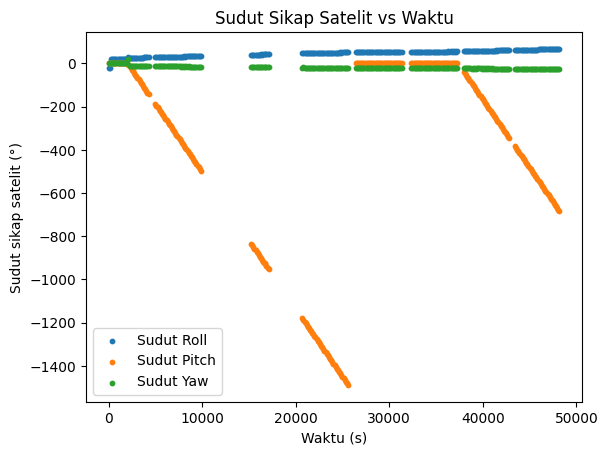
\includegraphics[width=0.7\textwidth]{fig/raw_angle_2018-05-19.png}
	\caption{Grafik sudut sikap satelit vs waktu pada 19 Mei 2018}
\label{fig:rawangle19}
\end{center}
\end{figure}

\begin{figure}[H]
\setlength\belowcaptionskip{-0.7\baselineskip}
\begin{center}
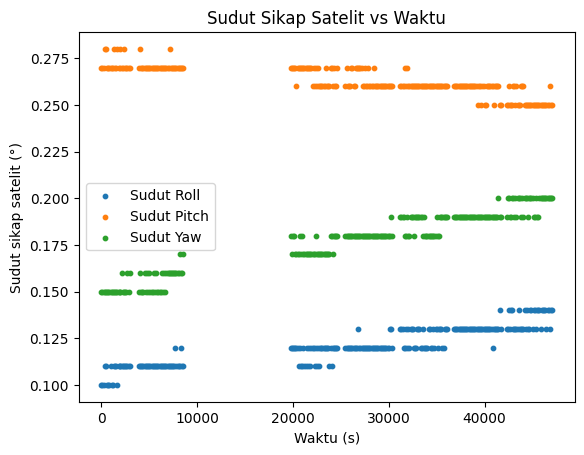
\includegraphics[width=0.7\textwidth]{fig/raw_angle_2018-05-20.png}
	\caption{Grafik sudut sikap satelit vs waktu pada 20 Mei 2018}
\label{fig:rawangle20}
\end{center}
\end{figure}

Selanjutnya, pengambilan data dilakukan selama kurun waktu sekitar 13 jam untuk
kedua periode observasi dengan selang waktu antar observasi satelit yang
bervariasi mulai dari puluhan detik sampai ribuan detik. Tabel
\ref{table:time19} dan \ref{table:time20} menunjukkan distribusi selang waktu
antar pengamatan pada kedua periode observasi. Dapat dilihat bahwa selang waktu
antar pengamatan didominasi oleh nilai 120 s dan disusul nilai 80 s.

\begin{table}[!ht]
\begin{center}
\caption{Distribusi selang waktu antar pengamatan satelit 19 Mei 2018}
\label{table:time19}
\begin{tabular}{|l|l|}
\hline
Selang waktu (s) & Frekuensi \\ \hline
80               & 8         \\ \hline
110              & 1         \\ \hline
120              & 289       \\ \hline
600              & 1         \\ \hline
720              & 2         \\ \hline
840              & 1         \\ \hline
1040             & 1         \\ \hline
3600             & 1         \\ \hline
5360             & 1         \\ \hline
\end{tabular}
\end{center}
\vspace{-5mm}
\end{table}

\begin{table}[!ht]
\begin{center}
\caption{Distribusi selang waktu antar pengamatan satelit 20 Mei 2018}
\label{table:time20}
\begin{tabular}{|l|l|}
\hline
Selang waktu (s) & Frekuensi \\ \hline
80               & 7         \\ \hline
120              & 260       \\ \hline
130              & 2         \\ \hline
600              & 1         \\ \hline
720              & 1         \\ \hline
840              & 2         \\ \hline
960              & 1         \\ \hline
11200            & 1         \\ \hline
\end{tabular}
\end{center}
\vspace{-5mm}
\end{table}

Terdapat jeda antar pengamatan satelit yang cukup besar pada kedua periode
observasi. Pada 19 Mei 2018, selang waktu antar pengamatan terbesar adalah 5360
s sedangkan pada 20 Mei 2018, selang waktu antar pengamatan maksimum mencapai
11200 s. Selang waktu tersebut sangat signifikan jika dibandingkan dengan
periode orbit satelit LAPAN-A3 sebesar 5700 s. 

Diketahui dari operator LAPAN bahwa LAPAN-A3 memiliki keterbatasan memori untuk
penyimpanan data telemetri sehingga hanya data telemetri selama 1 periode orbit
terakhir yang dapat diunduh. Selain itu, LAPAN juga memiliki satelit-satelit lain
dengan misi yang tidak kalah penting. Karena itu, jeda antar pengamatan satelit
LAPAN-A3 kemungkinan besar disebabkan pada waktu tersebut ada operasi satelit lain
yang lebih penting untuk diunduh oleh \textit{ground station} LAPAN.

Selain data telemetri satelit, data TLE LAPAN-A3 untuk kedua periode observasi
juga dikumpulkan. Data TLE satelit LAPAN-A3 yang digunakan sendiri dapat
dilihat pada Gambar \ref{fig:tlea3_mei19} dan \ref{fig:tlea3_mei20}. Nilai TLE
satelit diasumsikan tidak berubah selama 1 periode observasi. Karena itu,
\textit{epoch} atau waktu acuan yang digunakan untuk perhitungan orbit satelit
selama 1 hari pada bagian berikutnya adalah data TLE pertama yang tersedia pada
periode observasi sesuai zona waktu UTC. Asumsi ini didasari oleh algoritma
SGP-4 yang digunakan untuk mempropagasi orbit satelit LAPAN-A3 memiliki akurasi
yang cukup untuk memprediksi orbit satelit dalam rentang waktu 15 hari dari
waktu acuan \cite{kelsoa}. Secara spesifik untuk LAPAN-A3, selisih kesalahan
rata-rata perhitungan posisi LAPAN-A3 yang menggunakan data TLE terbaru dan
data TLE 1 hari sebelumnya bernilai 0.364 km \cite{nugroho2018}.

\begin{figure}[H]
\setlength\belowcaptionskip{-0.7\baselineskip}
\begin{center}
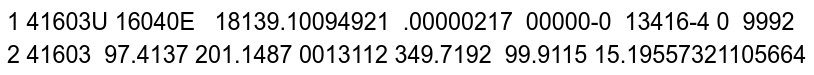
\includegraphics[width=0.7\textwidth]{fig/tlea3_2018-05-19.png}
\caption{Data TLE LAPAN-A3 pada 19 Mei 2018}
\label{fig:tlea3_mei19}
\end{center}
\end{figure}

\begin{figure}[H]
\setlength\belowcaptionskip{-0.7\baselineskip}
\begin{center}
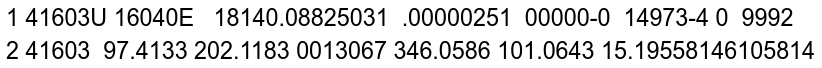
\includegraphics[width=0.7\textwidth]{fig/tlea3_2018-05-20.png}
\caption{Data TLE LAPAN-A3 pada 20 Mei 2018}
\label{fig:tlea3_mei20}
\end{center}
\end{figure}

\section{Pembuatan Dataset}

Sebagai gambaran umum, diagram alir yang ditunjukkan Gambar \ref{fig:algoritma}
pada bagian Metodologi memperlihatkan \textit{pipeline} data dalam pembuatan
dataset untuk model \textit{machine learning}. Pembuatan dataset dilakukan
dengan mempersiapkan dataset dasar, menghitung faktor termal satelit, dan
menyaring dataset.

\subsection{Persiapan Dataset Dasar}

Data mentah yang sudah dikumpulkan di tahap sebelumnya diproses terlebih dahulu
lewat kode Python sehingga memiliki bentuk dan satuan yang sesuai untuk
diproses lebih lanjut di tahap berikutnya. Proses ini dilakukan hanya pada data
mentah telemetri satelit LAPAN-A3 karena data TLE sudah dalam format yang dapat
digunakan oleh modul Skyfield. 

Pertama, data telemetri satelit mentah yang sudah diunduh diproses menggunakan modul Pandas sehingga hanya tersisa data telemetri satelit yang dibutuhkan. Selanjutnya, satuan data diubah menjadi satuan SI :

\begin{enumerate}
	\item Suhu \textit{node} dalam K
	\item Arus sensor Matahari \textit{node} dalam A
	\item Sudut sikap satelit dalam rad
\end{enumerate}

Kemudian, laju perubahan suhu \textit{node} juga dihitung dan data waktu
pembacaan sensor satelit dipisah menjadi format tahun, bulan, tanggal, jam,
menit, dan detik untuk memudahkan perhitungan faktor-faktor termal satelit di
bagian selanjutnya. Karena perubahan satuan untuk suhu \textit{node}, arus
sensor Matahari \textit{node}, dan sudut sikap satelit terjadi secara linear,
secara umum bentuk grafik ketiga jenis data tersebut tidak berubah. Dengan
begitu, hanya akan ditampilkan grafik laju perubahan suhu \textit{node} satelit
vs waktu yang dapat dilihat pada Gambar \ref{fig:basetempchange1219} sampai dengan
\ref{fig:basetempchange720}.

\begin{figure}[H]
\setlength\belowcaptionskip{-0.7\baselineskip}
\begin{center}
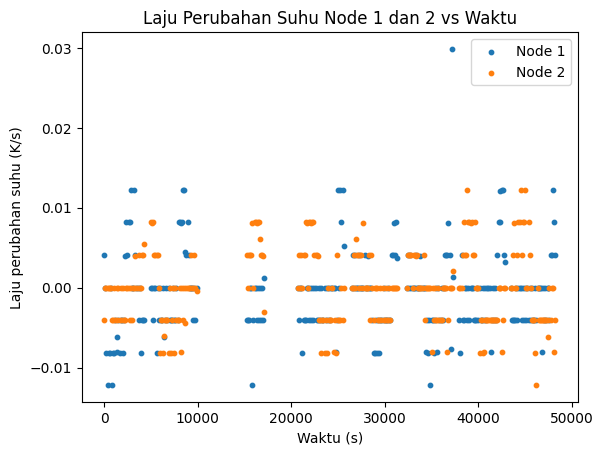
\includegraphics[width=0.7\textwidth]{fig/base_node12_tempchange_2018-05-19.png}
	\caption{Grafik laju perubahan suhu \textit{node} 1 dan 2 satelit vs waktu pada 19 Mei 2018}
\label{fig:basetempchange1219}
\end{center}
\end{figure}

\begin{figure}[H]
\setlength\belowcaptionskip{-0.7\baselineskip}
\begin{center}
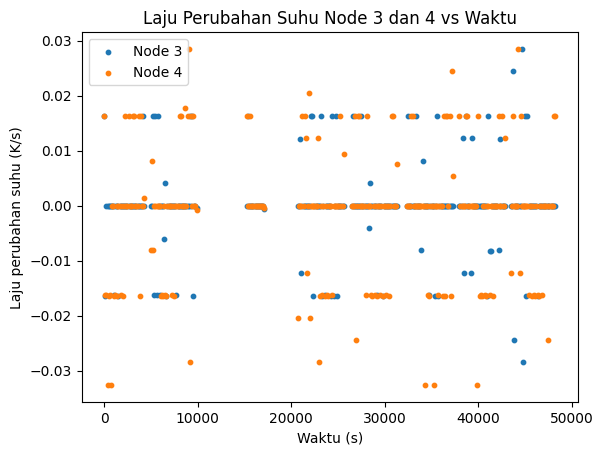
\includegraphics[width=0.7\textwidth]{fig/base_node34_tempchange_2018-05-19.png}
	\caption{Grafik laju perubahan suhu \textit{node} 3 dan 4 satelit vs waktu pada 19 Mei 2018}
\label{fig:basetempchange3419}
\end{center}
\end{figure}

\begin{figure}[H]
\setlength\belowcaptionskip{-0.7\baselineskip}
\begin{center}
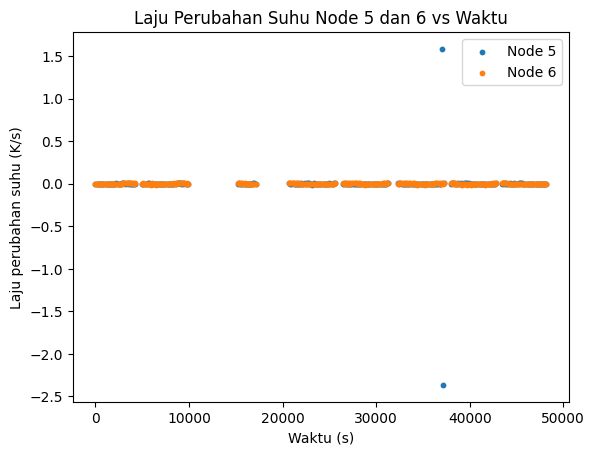
\includegraphics[width=0.7\textwidth]{fig/base_node56_tempchange_2018-05-19.png}
	\caption{Grafik laju perubahan suhu \textit{node} 5 dan 6 satelit vs waktu pada 19 Mei 2018}
\label{fig:basetempchange5619}
\end{center}
\end{figure}

\begin{figure}[H]
\setlength\belowcaptionskip{-0.7\baselineskip}
\begin{center}
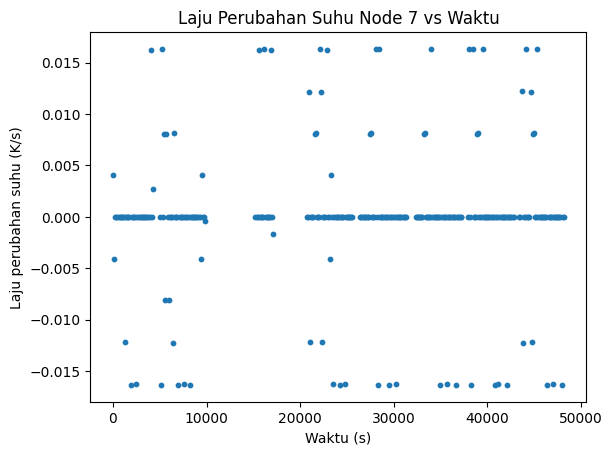
\includegraphics[width=0.7\textwidth]{fig/base_node7_tempchange_2018-05-19.png}
	\caption{Grafik laju perubahan suhu \textit{node} 7 satelit vs waktu pada 19 Mei 2018}
\label{fig:basetempchange719}
\end{center}
\end{figure}

\begin{figure}[H]
\setlength\belowcaptionskip{-0.7\baselineskip}
\begin{center}
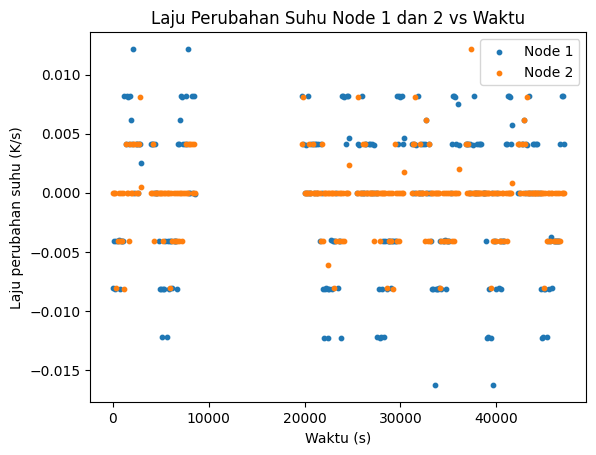
\includegraphics[width=0.7\textwidth]{fig/base_node12_tempchange_2018-05-20.png}
	\caption{Grafik laju perubahan suhu \textit{node} 1 dan 2 satelit vs waktu pada 20 Mei 2018}
\label{fig:basetempchange1220}
\end{center}
\end{figure}

\begin{figure}[H]
\setlength\belowcaptionskip{-0.7\baselineskip}
\begin{center}
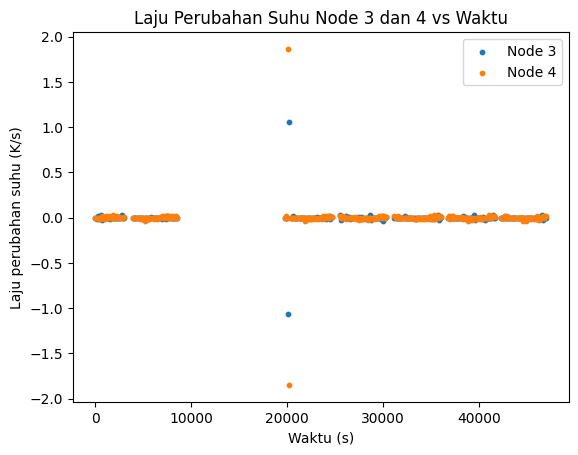
\includegraphics[width=0.7\textwidth]{fig/base_node34_tempchange_2018-05-20.png}
	\caption{Grafik laju perubahan suhu \textit{node} 3 dan 4 satelit vs waktu pada 20 Mei 2018}
\label{fig:basetempchange3420}
\end{center}
\end{figure}

\begin{figure}[H]
\setlength\belowcaptionskip{-0.7\baselineskip}
\begin{center}
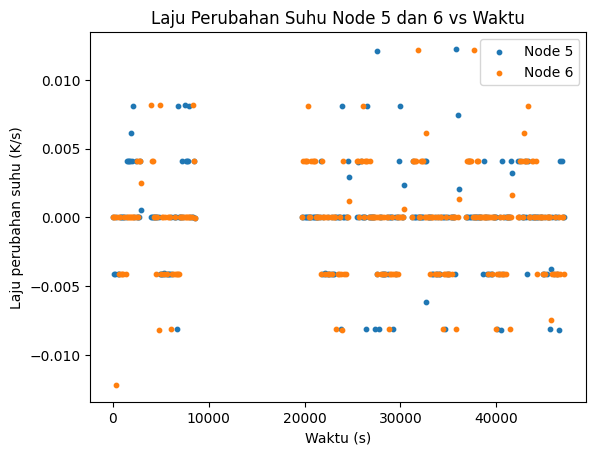
\includegraphics[width=0.7\textwidth]{fig/base_node56_tempchange_2018-05-20.png}
	\caption{Grafik laju perubahan suhu \textit{node} 5 dan 6 satelit vs waktu pada 20 Mei 2018}
\label{fig:basetempchange5620}
\end{center}
\end{figure}

\begin{figure}[H]
\setlength\belowcaptionskip{-0.7\baselineskip}
\begin{center}
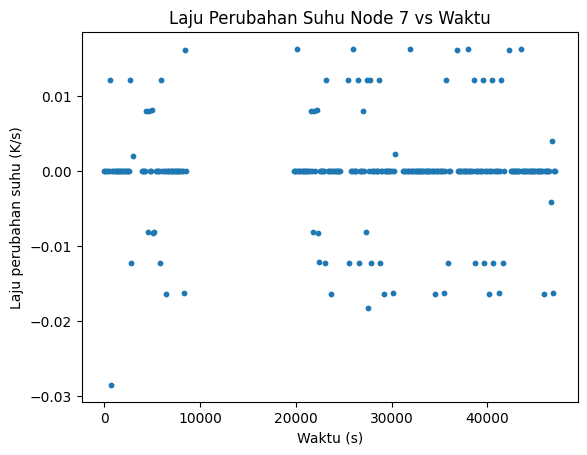
\includegraphics[width=0.7\textwidth]{fig/base_node7_tempchange_2018-05-20.png}
	\caption{Grafik laju perubahan suhu \textit{node} 7 satelit vs waktu pada 20 Mei 2018}
\label{fig:basetempchange720}
\end{center}
\end{figure}

\subsection{Perhitungan Faktor Termal Satelit}

Sesuai diagram alir \textit{pipeline} yang ditunjukkan Gambar
\ref{fig:algoritma} dan tabel variabel yang masih belum diketahui pada Tabel
\ref{table:unknown}, perhitungan faktor termal satelit terbagi mencakup 3 jenis
variabel : faktor panas akibat Matahari, Bumi, dan albedo. Ketiga jenis
variabel tersebut dihitung juga menggunakan kode Python.

Karena \textit{node} 7 pada model satelit LAPAN-A3 mewakili plat tengah satelit
yang diasumsikan terisolasi dari lingkungan luar satelit, laju perubahan suhu
\textit{node} 7 dianggap tidak dipengaruhi faktor panas akibat Matahari,
albedo, maupun Bumi. Diasumsikan juga \textit{node} 7 tidak mengalami disipasi
panas ke lingkungan ruang angkasa sehingga perubahan suhu pada \textit{node} 7
murni terjadi akibat perpindahan panas lewat konduksi dan radiasi dengan
ke-enam \textit{node} lainnya. Dengan demikian, ketiga jenis variabel hanya
akan dihitung untuk \textit{node} 1 sampai dengan 6.


\subsubsection{Faktor Panas Akibat Matahari}

Faktor panas akibat Matahari merupakan hasil perkalian bacaan arus sensor
Matahari \textit{node} dan faktor gerhana \textit{node} satelit. Bacaan arus
sensor Matahari sudah dihitung pada tahap Persiapan Dataset Dasar. Sejalan
dengan definisi faktor gerhana node yang dijelaskan pada bab Tinjauan Pustaka,
nilai variabel tersebut dapat ditentukan dari pembacaan arus sensor sinar
Matahari \textit{node} terkait; bacaan arus lebih besar dari 0 A berarti
\textit{node} menerima sinar Matahari sehingga memiliki nilai faktor gerhana
sebesar 1. Sebaliknya, jika bacaan arus sensor \textit{node} bernilai 0,
\textit{node} tidak menerima sinar Matahari sehingga memiliki nilai faktor
gerhana 0.

Perhitungan faktor gerhana \textit{node} dari data arus sensor Matahari
\textit{node} harus memperhatikan toleransi kesalahan bacaan sensor yang
mungkin terjadi. Sebagai contoh, sensor Matahari pada satelit LAPAN-A3 yang
digunakan dalam karya tulis ini menunjukkan pembacaan lebih besar dari 0 A pada
beberapa selang waktu pengamatan meskipun seharusnya satelit berada pada fase
gerhana mengikuti pada nilai bacaan arus sensor \textit{node} selang waktu
sebelum dan sesudahnya. Bacaan arus sensor Matahari \textit{node} tersebut
dapat dianggap sebagai kesalahan instrumen pengukuran karena terjadi konsisten
pada setiap sensor dengan besar yang sama dan hanya terjadi pada beberapa
selang waktu tertentu saat satelit jelas dalam fase gerhana.

Gambar \ref{fig:solar1219} sampai dengan \ref{fig:solar5620} menunjukkan hasil
perhitungan faktor panas akibat Matahari \textit{node} satelit LAPAN-A3. Dapat dilihat bahwa grafik faktor panas akibat Matahari memiliki bentuk yang hampir sama dengan grafik arus sensor Matahari \textit{node} satelit.

\begin{figure}[H]
\setlength\belowcaptionskip{-0.7\baselineskip}
\begin{center}
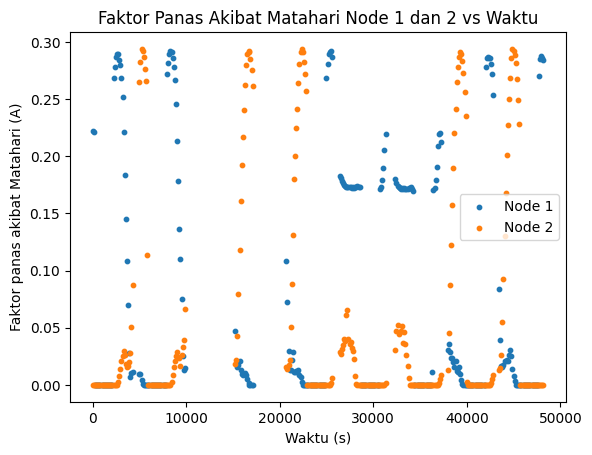
\includegraphics[width=0.7\textwidth]{fig/solar_node12_2018-05-19.png}
	\caption{Grafik faktor panas akibat Matahari \textit{node} 1 dan 2 satelit vs waktu pada 19 Mei 2018}
\label{fig:solar1219}
\end{center}
\end{figure}

\begin{figure}[H]
\setlength\belowcaptionskip{-0.7\baselineskip}
\begin{center}
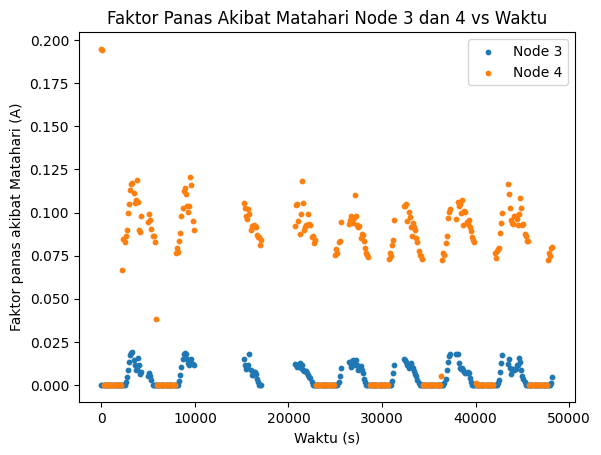
\includegraphics[width=0.7\textwidth]{fig/solar_node34_2018-05-19.png}
	\caption{Grafik faktor panas akibat Matahari \textit{node} 3 dan 4 satelit vs waktu pada 19 Mei 2018}
\label{fig:solar3419}
\end{center}
\end{figure}

\begin{figure}[H]
\setlength\belowcaptionskip{-0.7\baselineskip}
\begin{center}
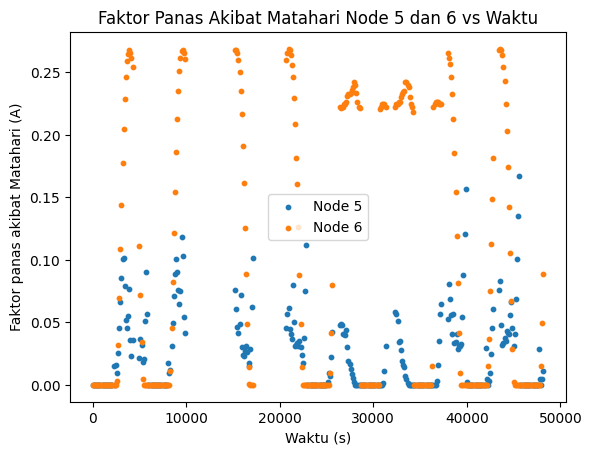
\includegraphics[width=0.7\textwidth]{fig/solar_node56_2018-05-19.png}
	\caption{Grafik faktor panas akibat Matahari \textit{node} 5 dan 6 satelit vs waktu pada 19 Mei 2018}
\label{fig:solar5619}
\end{center}
\end{figure}

\begin{figure}[H]
\setlength\belowcaptionskip{-0.7\baselineskip}
\begin{center}
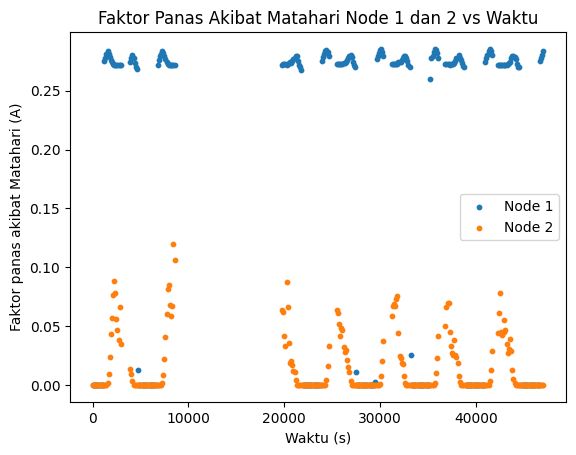
\includegraphics[width=0.7\textwidth]{fig/solar_node12_2018-05-20.png}
	\caption{Grafik faktor panas akibat Matahari \textit{node} 1 dan 2 satelit vs waktu pada 20 Mei 2018}
\label{fig:solar1220}
\end{center}
\end{figure}

\begin{figure}[H]
\setlength\belowcaptionskip{-0.7\baselineskip}
\begin{center}
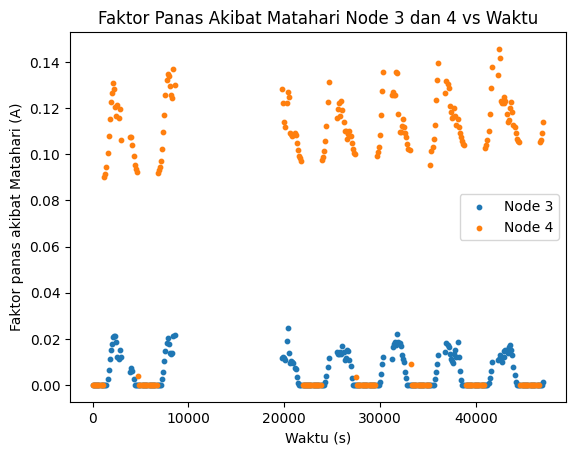
\includegraphics[width=0.7\textwidth]{fig/solar_node34_2018-05-20.png}
	\caption{Grafik faktor panas akibat Matahari \textit{node} 3 dan 4 satelit vs waktu pada 20 Mei 2018}
\label{fig:solar3420}
\end{center}
\end{figure}

\begin{figure}[H]
\setlength\belowcaptionskip{-0.7\baselineskip}
\begin{center}
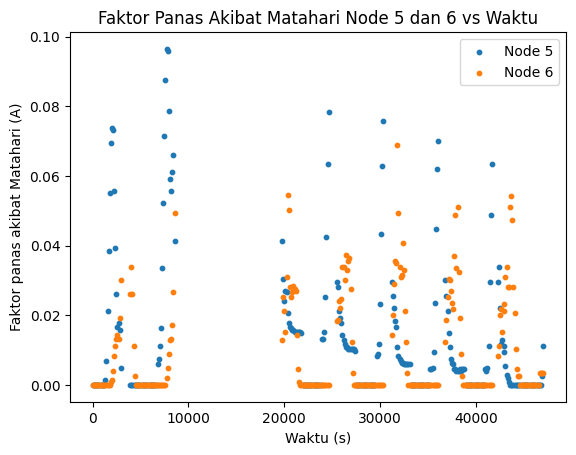
\includegraphics[width=0.7\textwidth]{fig/solar_node56_2018-05-20.png}
	\caption{Grafik faktor panas akibat Matahari \textit{node} 5 dan 6 satelit vs waktu pada 20 Mei 2018}
\label{fig:solar5620}
\end{center}
\end{figure}

\subsubsection{Faktor Panas Akibat Bumi}

Faktor panas akibat Bumi dan albedo sama-sama bergantung pada perhitungan
\textit{view factor} \textit{node} satelit ke Bumi. Sesuai dengan Persamaan
\ref{eq:vf}, \textit{view factor} dari \textit{node} satelit ke Bumi didekati
dengan \textit{view factor} dari plat persegi panjang ke bola. Persamaan
\ref{eq:vf} membutuhkan jari-jari bola $r$, jarak antara plat dengan bola $R$,
dan sudut antara garis normal permukaan plat dengan garis jarak antara plat dan
bola $\gamma$. 

Jari-jari bola $r$ dapat didekati dengan nilai rata-rata jari-jari Bumi sebesar
6371 km \cite{moritz}. Lalu, karena ukuran satelit jauh lebih kecil dari Bumi,
jarak plat ke bola $H$ dapat didekati dengan jarak antara satelit dan Bumi yang
dapat dihitung dengan mempropagasi orbit satelit berdasarkan data TLE
menggunakan modul Skyfield. Propagasi orbit lewat modul Skyfield juga
memungkinkan perhitungan vektor posisi satelit seiring perubahan waktu. Dengan
demikian, sudut antara garis normal permukaan plat dengan bola $\gamma$ dapat
didekati dengan sudut antara vektor normal permukaan \textit{node} dengan
vektor posisi satelit terhadap Bumi. 

Perhitungan sudut $\gamma$ perlu memperhatikan tata acuan koordinat yang
digunakan pada kedua vektor. Vektor posisi satelit terhadap Bumi yang dihitung
dengan modul Skyfield dinyatakan dalam \textit{Geocentric Celestial
Reference System} (GCRS). GCRS merupakan pengembangan lebih lanjut tata acuan
koordinat inersial Bumi seperti yang ditunjukkan sumbu $\hat{x}_i$,
$\hat{y}_i$, dan $\hat{z}_i$ pada Gambar \ref{fig:referenceframe}.

\begin{figure}[H]
\setlength\belowcaptionskip{-0.7\baselineskip}
\begin{center}
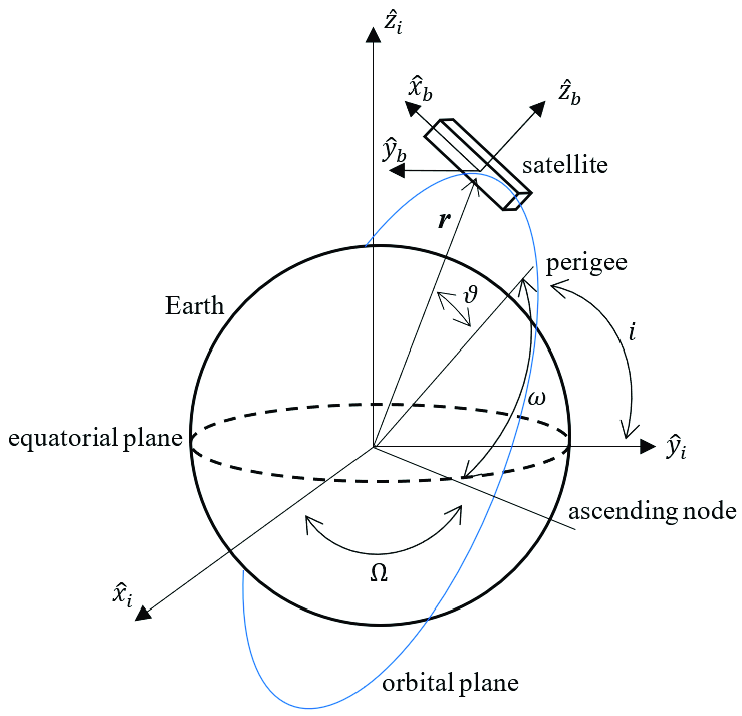
\includegraphics[width=0.7\textwidth]{fig/referenceframe.png}
	\caption[Ilustrasi sistem koordinat satelit yang mengorbit Bumi]{Ilustrasi sistem koordinat satelit yang mengorbit Bumi~\cite{farissi2019}}
\label{fig:referenceframe}
\end{center}
\end{figure}

Sementara itu, vektor normal permukaan \textit{node} satelit masih dinyatakan
dalam sistem koordinat badan satelit seperti yang ditunjukkan $\hat{x}_b$,
$\hat{y}_b$, dan $\hat{z}_b$ pada Gambar \ref{fig:referenceframe}. Karena itu, vektor normal permukaan \textit{node}
harus dikonversi terlebih dahulu dengan bantuan matriks rotasi sudut Euler
dengan urutan Z-Y-X menjadi dalam bentuk tata acuan koordinat inersial Bumi.
Setelah itu, nilai \textit{view factor node} satelit dapat dihitung. 

Faktor panas akibat Bumi \textit{node} satelit kemudian dapat dicari dengan
mengalikan \textit{view factor node} dengan suhu \textit{node} pangkat 4.
Gambar \ref{fig:earth1219} sampai dengan \ref{fig:earth5620} menunjukkan hasil
perhitungan faktor panas akibat Bumi. Dapat dilihat bahwa sisi-sisi satelit
yang berlawanan memiliki tren nilai faktor panas akibat Bumi yang berlawanan
juga. Dengan kata lain saat sebuah \textit{node} memiliki nilai faktor panas
akibat Bumi yang maksimum, \textit{node} satelit di sisi yang berlawanan dengan
\textit{node} tersebut memiliki nilai faktor panas minimum. Hal ini terjadi
karena saat suatu sisi satelit mendekati atau tepat menghadap ke  permukaan Bumi
(\textit{view factor node} mendekati nilai 1), sisi satelit yang berlawanan akan memiliki nilai \textit{view factor} mendekati 0.

\begin{figure}[H]
\setlength\belowcaptionskip{-0.7\baselineskip}
\begin{center}
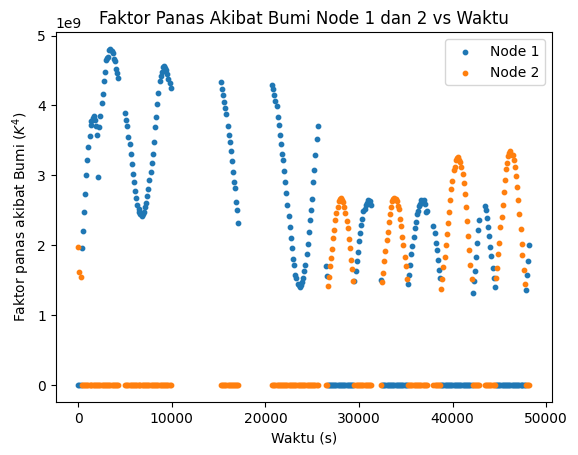
\includegraphics[width=0.7\textwidth]{fig/earth_node12_2018-05-19.png}
	\caption{Grafik faktor panas akibat Bumi \textit{node} 1 dan 2 satelit vs waktu pada 19 Mei 2018}
\label{fig:earth1219}
\end{center}
\end{figure}

\begin{figure}[H]
\setlength\belowcaptionskip{-0.7\baselineskip}
\begin{center}
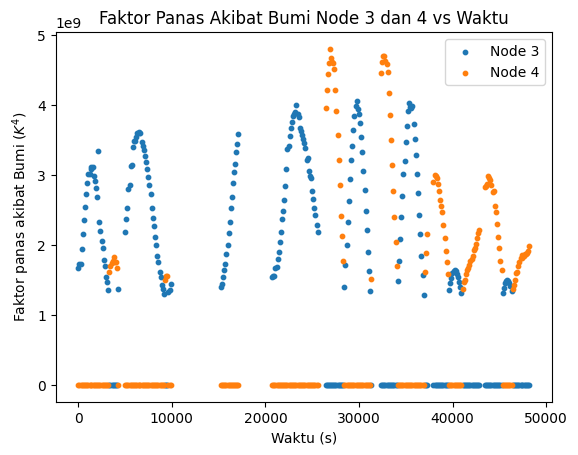
\includegraphics[width=0.7\textwidth]{fig/earth_node34_2018-05-19.png}
	\caption{Grafik faktor panas akibat Bumi \textit{node} 3 dan 4 satelit vs waktu pada 19 Mei 2018}
\label{fig:earth3419}
\end{center}
\end{figure}

\begin{figure}[H]
\setlength\belowcaptionskip{-0.7\baselineskip}
\begin{center}
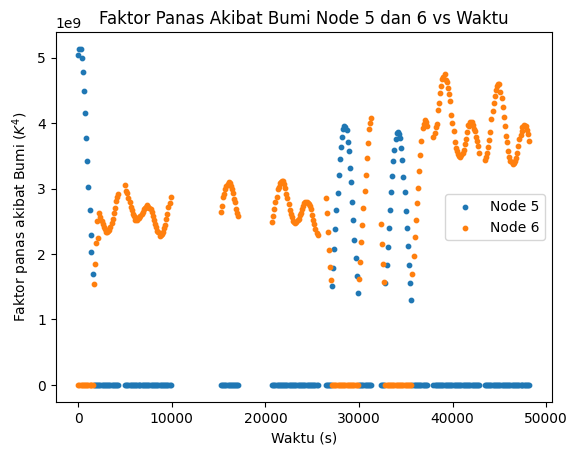
\includegraphics[width=0.7\textwidth]{fig/earth_node56_2018-05-19.png}
	\caption{Grafik faktor panas akibat Bumi \textit{node} 5 dan 6 satelit vs waktu pada 19 Mei 2018}
\label{fig:earth5619}
\end{center}
\end{figure}

\begin{figure}[H]
\setlength\belowcaptionskip{-0.7\baselineskip}
\begin{center}
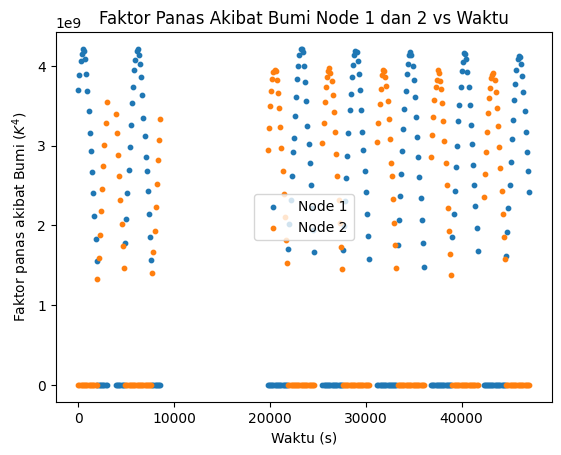
\includegraphics[width=0.7\textwidth]{fig/earth_node12_2018-05-20.png}
	\caption{Grafik faktor panas akibat Bumi \textit{node} 1 dan 2 satelit vs waktu pada 20 Mei 2018}
\label{fig:earth1220}
\end{center}
\end{figure}

\begin{figure}[H]
\setlength\belowcaptionskip{-0.7\baselineskip}
\begin{center}
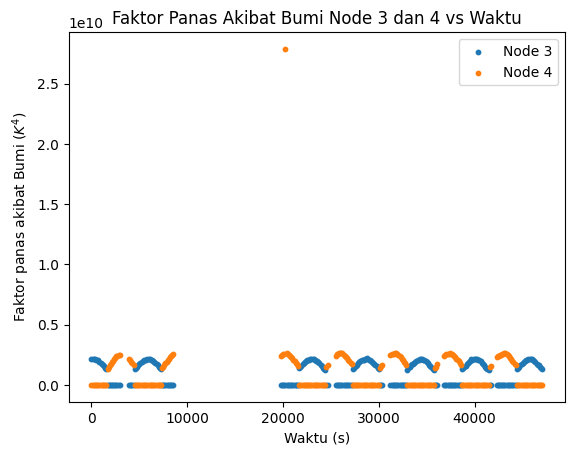
\includegraphics[width=0.7\textwidth]{fig/earth_node34_2018-05-20.png}
	\caption{Grafik faktor panas akibat Bumi \textit{node} 3 dan 4 satelit vs waktu pada 20 Mei 2018}
\label{fig:earth3420}
\end{center}
\end{figure}

\begin{figure}[H]
\setlength\belowcaptionskip{-0.7\baselineskip}
\begin{center}
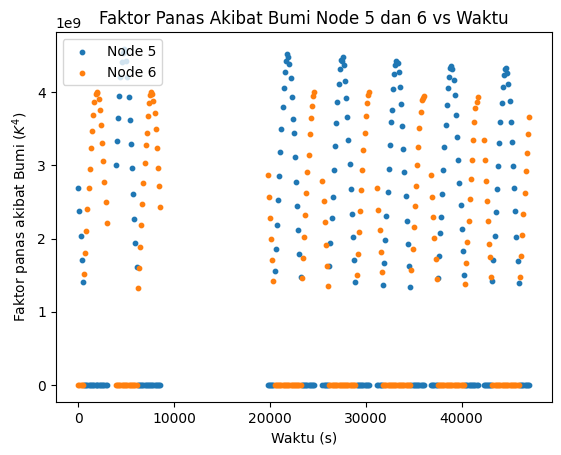
\includegraphics[width=0.7\textwidth]{fig/earth_node56_2018-05-20.png}
	\caption{Grafik faktor panas akibat Bumi \textit{node} 5 dan 6 satelit vs waktu pada 20 Mei 2018}
\label{fig:earth5620}
\end{center}
\end{figure}

\subsubsection{Faktor Panas Akibat Albedo}

Perhitungan faktor panas akibat albedo membutuhkan faktor albedo satelit.
Sesuai dengan Persamaan \ref{eq:albedofactor}, nilai faktor albedo satelit
bergantung pada faktor gerhana satelit serta posisi sudut satelit dan mulainya
fase gerhana terhadap titik \textit{sub-solar}. Sama dengan perhitungan faktor
gerhana \textit{node}, faktor gerhana satelit akan bernilai 1 saat satelit
menerima sinar Matahari dan bernilai 0 saat satelit berada pada fase gerhana.
Dengan demikian, faktor gerhana satelit bernilai 0 saat semua \textit{node}
satelit memiliki faktor gerhana 0 dan bernilai 1 jika ada 1 atau lebih
\textit{node} yang memiliki faktor gerhana 1.

Untuk mencari posisi sudut satelit dan mulainya fase gerhana terhadap titik
\textit{sub-solar}, perlu dihitung terlebih dahulu nilai anomali benar satelit
fase gerhana mulai dan berakhir. Nilai anomali benar satelit dapat dicari lewat
propagasi orbit menggunakan modul Skyfield berdasarkan data TLE sesuai data
waktu satelit dari data telemetri satelit. Dengan mengasumsikan simetri orbit
lingkaran sehingga titik \textit{sub-solar} berada di tengah titik akhir dan mulai fase gerhana satelit seperti yang ditunjukkan lokasi \textit{conjunction point} pada Gambar \ref{fig:ssp}, anomali benar titik \textit{sub-solar} dapat dihitung.

\begin{figure}[H]
\setlength\belowcaptionskip{-0.7\baselineskip}
\begin{center}
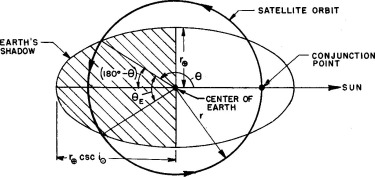
\includegraphics[width=0.6\textwidth]{fig/ssp.jpg}
	\caption[Ilustrasi fase gerhana pada orbit satelit]{Ilustrasi fase gerhana pada orbit satelit~\cite{ismail2015}}
\label{fig:ssp}
\end{center}
\end{figure}

Selanjutnya, posisi sudut satelit terhadap titik \textit{sub-solar} untuk waktu
tertentu dapat dicari dengan mengurangi anomali benar satelit dengan anomali
benar titik \textit{sub-solar}. Kemudian, faktor panas akibat albedo dapat
dihitung dengan mengalikan \textit{view factor node} satelit dengan faktor
albedo satelit. Gambar \ref{fig:albedo1219} sampai dengan \ref{fig:albedo5620}
menunjukkan grafik faktor panas akibat albedo \textit{node} satelit vs waktu.

\begin{figure}[H]
\setlength\belowcaptionskip{-0.7\baselineskip}
\begin{center}
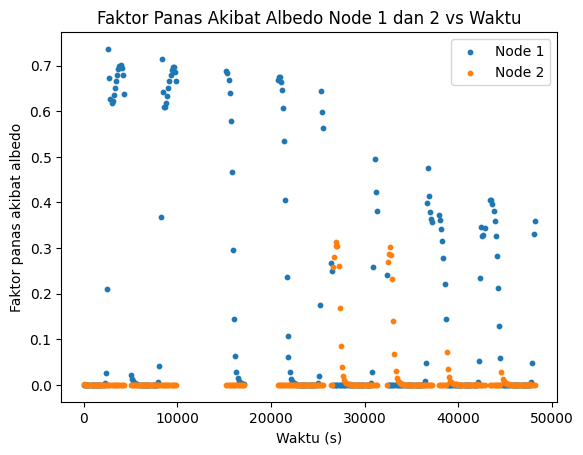
\includegraphics[width=0.7\textwidth]{fig/albedo_node12_2018-05-19.png}
	\caption{Grafik faktor panas akibat albedo \textit{node} 1 dan 2 satelit vs waktu pada 19 Mei 2018}
\label{fig:albedo1219}
\end{center}
\end{figure}

\begin{figure}[H]
\setlength\belowcaptionskip{-0.7\baselineskip}
\begin{center}
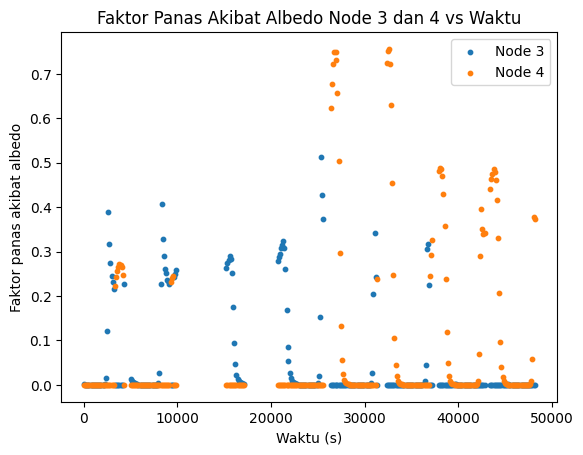
\includegraphics[width=0.7\textwidth]{fig/albedo_node34_2018-05-19.png}
	\caption{Grafik faktor panas akibat albedo \textit{node} 3 dan 4 satelit vs waktu pada 19 Mei 2018}
\label{fig:albedo3419}
\end{center}
\end{figure}

\begin{figure}[H]
\setlength\belowcaptionskip{-0.7\baselineskip}
\begin{center}
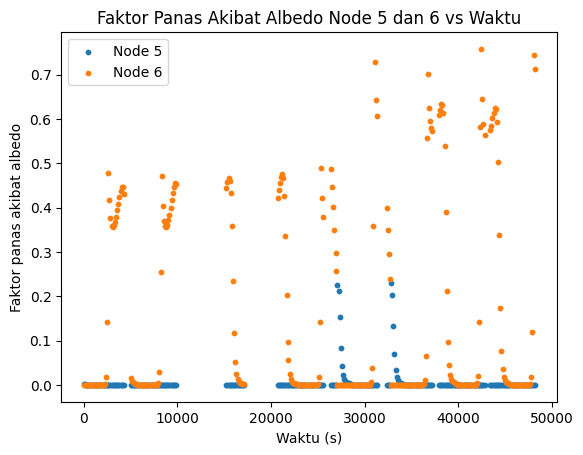
\includegraphics[width=0.7\textwidth]{fig/albedo_node56_2018-05-19.png}
	\caption{Grafik faktor panas akibat albedo \textit{node} 5 dan 6 satelit vs waktu pada 19 Mei 2018}
\label{fig:albedo5619}
\end{center}
\end{figure}

\begin{figure}[H]
\setlength\belowcaptionskip{-0.7\baselineskip}
\begin{center}
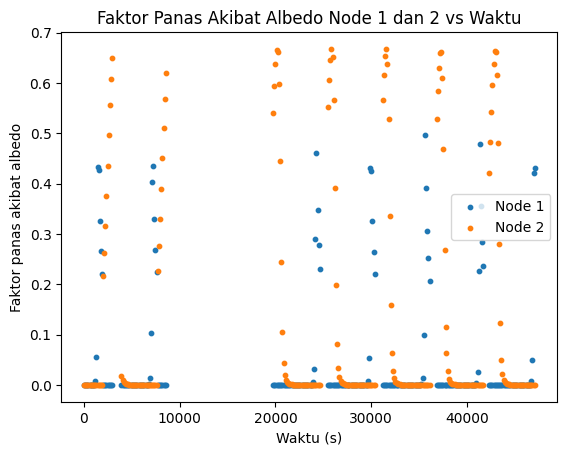
\includegraphics[width=0.7\textwidth]{fig/albedo_node12_2018-05-20.png}
	\caption{Grafik faktor panas akibat albedo \textit{node} 1 dan 2 satelit vs waktu pada 20 Mei 2018}
\label{fig:albedo1220}
\end{center}
\end{figure}

\begin{figure}[H]
\setlength\belowcaptionskip{-0.7\baselineskip}
\begin{center}
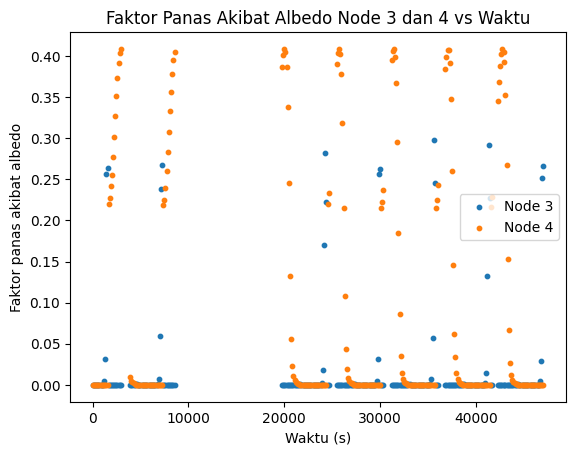
\includegraphics[width=0.7\textwidth]{fig/albedo_node34_2018-05-20.png}
	\caption{Grafik faktor panas akibat albedo \textit{node} 3 dan 4 satelit vs waktu pada 20 Mei 2018}
\label{fig:albedo3420}
\end{center}
\end{figure}

\begin{figure}[H]
\setlength\belowcaptionskip{-0.7\baselineskip}
\begin{center}
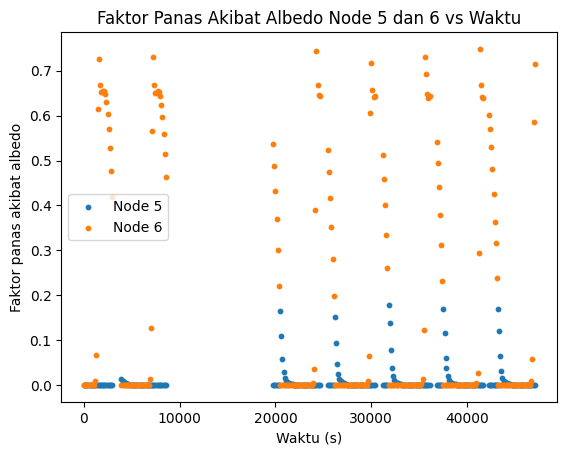
\includegraphics[width=0.7\textwidth]{fig/albedo_node56_2018-05-20.png}
	\caption{Grafik faktor panas akibat albedo \textit{node} 5 dan 6 satelit vs waktu pada 20 Mei 2018}
\label{fig:albedo5620}
\end{center}
\end{figure}

\subsection{Penyaringan dataset}

Data gabungan dataset dasar dan hasil perhitungan koefisien faktor termal
satelit kemudian disaring untuk menimalkan sumber ketidakuratan model regresi
linear. Sumber ketidakuratan pertama adalah selang waktu antar pengamatan yang
terlalu lama. Seperti yang sudah ditampilkan pada Tabel \ref{table:time19} dan
\ref{table:time20}, nilai selang waktu pengamatan bervariasi pada kedua periode
observasi. Seperti yang dapat dilihat pada grafik-grafik suhu \textit{node} satelit, suhu \textit{node} satelit berubah secara periodik sedangkan perubahan suhu \textit{node} satelit didekati secara linear. Karena itu, selang waktu antar pengamatan yang terlalu lama akan mengurangi akurasi prediksi model.

Selanjutnya, kesalahan pengukuran juga dapat mengurangi akurasi model. Salah
satu karakteristik dataset yang diasumsikan metode regresi linear adalah
dataset bebas dari kesalahan pengukuran. Pada nyatanya, sensor-sensor satelit
memiliki ketidakakuratan pengukuran inheren. Kesalahan pengukuran tersebut
dapat diperparah gangguan atau \textit{noise} yang secara alamiah terdapat pada
lingkungan ruang angkasa. Sebagai contoh, bacaan arus sensor Matahari
\textit{node} menunjukkan nilai lebih besar dari 0 A meski satelit berada pada
fase gerhana. Keberadaan kesalahan pengukuran akan mengurangi akurasi prediksi
regresi sehingga harus dihilangkan atau diminimalkan.

Dampak ketidakakuratan pengukuran dapat berakibat pada \textit{outlier}, poin
data yang jauh berbeda jika dibandingkan data lainnya. Secara visual, contoh
\textit{outlier} di data telemetri satelit LAPAN-A3 dapat dilihat pada Gambar
\ref{fig:outliertemp} dan \ref{fig:outliertempchange}. Gambar
\ref{fig:outliertemp} menunjukkan \textit{outlier} suhu \textit{node} 3 dan 4
pada 20 Mei 2018 sedangkan Gambar \ref{fig:outliertempchange} memperlihatkan
\textit{outlier} laju perubahan suhu \textit{node} 5 dan 6 pada 19 Mei
2018. Pada kedua gambar, terdapat poin-poin data yang jauh berbeda jika
dibandingkan dengan poin-poin data lainnya.

\begin{figure}[H]
\setlength\belowcaptionskip{-0.7\baselineskip}
\begin{center}
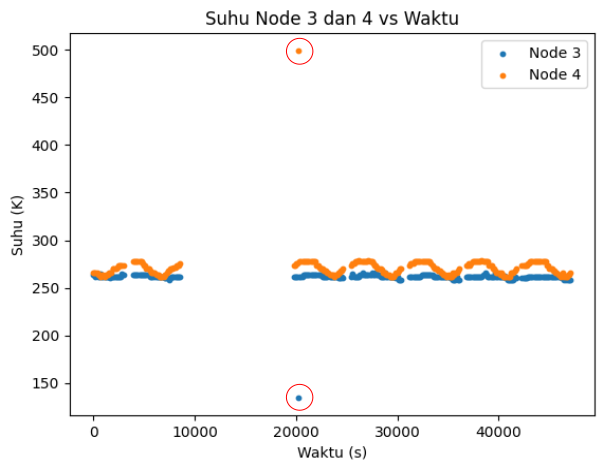
\includegraphics[width=0.7\textwidth]{fig/outliertemp.png}
	\caption{Poin \textit{outlier} di grafik suhu \textit{node} 3 dan 4 satelit vs waktu pada 20 Mei 2018}
\label{fig:outliertemp}
\end{center}
\end{figure}

\begin{figure}[H]
\setlength\belowcaptionskip{-0.7\baselineskip}
\begin{center}
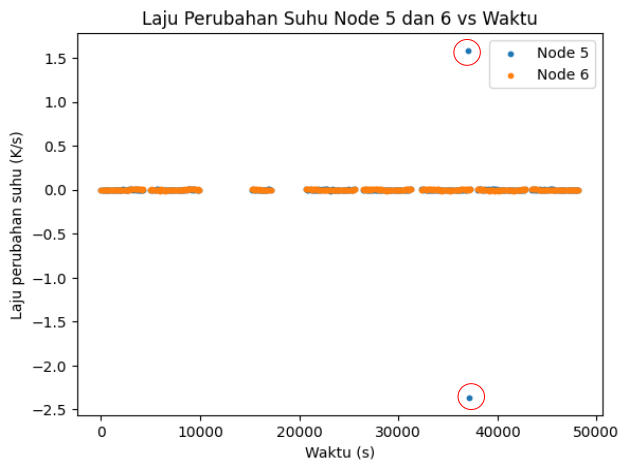
\includegraphics[width=0.7\textwidth]{fig/outliertempchange.png}
	\caption{Poin \textit{outlier} di grafik laju perubahan suhu \textit{node} 5 dan 6 satelit vs waktu pada 20 Mei 2018}
\label{fig:outliertempchange}
\end{center}
\end{figure}

Keberadaan \textit{outlier} juga dapat memperburuk akurasi model. Karena itu, \textit{outlier} harus dihilangkan dari dataset yang akan digunakan untuk model \textit{machine learning}.

Berdasarkan pertimbangan yang sudah dijelaskan, kriteria yang digunakan untuk
menyaring dataset adalah sebagai berikut :

\begin{enumerate}
\item Selang waktu antar pengamatan maksimal 120 s 
\item Skor standar suhu \textit{node} satelit memiliki rentang -3 sampai dengan 3
\item Skor standar laju perubahan suhu \textit{node} satelit berkisar dari -3 sampai dengan 3 
\end{enumerate}

Kriteria pertama dipilih berdasarkan persebaran selang waktu pengamatan untuk
data dari kedua periode observasi. Pada kedua periode observasi, mayoritas selang waktu pengamatan bernilai 120 s disusul dengan nilai 80 s. Karena itu, nilai 120 s akan dijadikan batas atas selang waktu pengamatan.

Kriteria kedua dan ketiga dipilih untuk menghilangkan \textit{outlier}
pembacaan sensor satelit. Secara statistik, salah satu cara untuk mengukur
apakah sebuah poin data termasuk dalam kategori \textit{outlier} adalah dengan
menghitung skor standar poin data tersebut. Skor standar $z$ dihitung dengan
membagi selisih antara nilai data $x$ dan rata-rata data $\mu$ dengan standar
deviasi data $\sigma$ seperti pada persamaan berikut \cite{massaron}:

\begin{equation}
\label{eq:zscore}
	z = \frac{x - \mu}{\sigma}
\end{equation}

Skor standar yang terlalu rendah (lebih kecil dari -3) atau tinggi (lebih besar
dari 3) mengindikasikan poin data tersebut dapat dikategorikan \textit{outlier}
\cite{boschetti2015}. Kedua kriteria skor standar mengasumsikan suhu dan laju
perubahan suhu \textit{node-node} satelit terdistribusi secara normal sesuai
dengan asumsi dasar pemodelan regresi linear dalam \textit{machine learning}.
Secara fisik, poin data dengan skor standar lebih kecil dari -3 atau lebih
tinggi dari 3 memiliki jarak lebih besar 3 kali standar deviasi dataset dari
rata-rata dataset. Dengan asumsi data terdistribusi secara normal, poin data
dengan skor standar di luar rentang -3 sampai dengan 3 poin data yang sangat
ekstrem dan jauh berbeda jika dibandingkan dengan poin-poin data lainnya. Ini
berarti poin data tersebut memiliki kemungkinan termasuk \textit{outlier}. 

Nilai \textit{outlier} dapat disebabkan oleh kesalahan pengukuran atau juga
dapat terjadi secara alamiah. Pada konteks data telemetri satelit LAPAN-A3,
\textit{outlier} yang terdeteksi dapat diduga terjadi akibat kesalahan
pengukuran karena nilai poin-poin data tersebut di luar rentang nilai
operasional sensor satelit. Sebagai contoh, bacaan sensor suhu \textit{outlier}
pada Gambar \ref{fig:outliertemp} mendekati nilai 500 K dan kemudian langsung
berubah menjadi rentang suhu yang wajar pada selang waktu berikutnya. Jika suhu
satelit benar-benar mencapai nilai tersebut, tentunya satelit sudah mengalami
kerusakan permanen.

\section{Pengaturan Model Machine Learning}

Seperti yang sudah dijelakan pada bab Tinjauan Pustaka, ada beberapa metode
pendekatan regresi linear dalam metode \textit{machine learning} yang dapat
digunakan untuk menyelesaikan persamaan termal satelit. Ketiga pendekatan
regresi linear juga sudah tersedia pada modul Scikit-learn sehingga tidak perlu
diimplementasikan dari awal. Pemodelan pada karya tulis ini menggunakan
pendekatan regresi linear OLS untuk menghitung variabel-variabel termal satelit
yang tidak diketahui. Pendekatan OLS dipilih karena beberapa alasan dan
pertimbangan terkait data telemetri satelit dan model termal yang akan dibuat. 

Pertama, pendekatan OLS adalah pendekatan paling sederhana untuk menyelesaikan
persamaan regresi linear. Berbeda dengan pendekatan regresi linear lainnya,
pendekatan ini tidak membutuhkan asumsi maupun pengetahuan tambahan mengenai
dataset yang akan dianalisis. Jika ditemukan bahwa performa model regresi
linear menggunakan OLS tidak mencapai tingkat akurasi yang diinginkan, evaluasi
yang dilakukan dapat menjadi bahan pertimbangan untuk menganalisis
karakteristik dataset pada pengembangan model termal selanjutnya. Sebaliknya,
jika performa model regresi linear OLS sudah memenuhi tingkat akurasi yang
diinginkan, analisis lebih lanjut pada hasil pemodelan tersebut dapat memberi
petunjuk untuk meningkatkan performa model termal di masa depan.

Selanjutnya, pendekatan OLS tidak membutuhkan pengaturan \textit{hyperparameter}
(parameter \textit{machine learning} yang mengatur jalannya proses pelatihan
model) seperti yang dibutuhkan pendekatan PLS dan RLS. Pendekatan PLS
membutuhkan \textit{hyperparameter} untuk menentukan jumlah variabel independen
yang akan digunakan sedangkan RLS membutuhkan \textit{hyperparameter} untuk
menentukan nilai koefisien regularisasi $k$. Keberadaan \textit{hyperparameter}
mengharuskan pembagian dataset menjadi set latihan, \textit{cross-validation},
dan ujian karena nilai optimum \textit{hyperparameter} dicari pada tahap
\textit{cross-validation}.

Pembagian data menjadi 3 kategori akan mengurangi jumlah data yang tersedia
untuk tahap pelatihan dan pengujian sedangkan dataset mentah yang tersedia dari
kedua periode observasi hanya berkisar di rentang 280-300 poin data akibat
adanya jeda observasi yang cukup lama. Jumlah data tersebut adalah jumlah data
mentah yang belum disaring sehingga jumlah data final yang akan digunakan model
tentunya lebih sedikit dari jumlah awal tersebut. Lebih lanjut, karena tujuan utama
dari model termal pada karya tulis ini adalah prediksi, keuntungan penggunaan
PLS dan RLS yang resilien terhadap kolinearitas tidak berdampak banyak pada
akurasi prediksi model \cite{lieberman2014}\cite{mundfrom2018}.

Terakhir, metode OLS lazim digunakan sebagai referensi \textit{baseline}
performa model regresi linear. Dengan demikian, jika performa model termal
dengan regresi linear OLS sudah diketahui, pengembangan model termal satelit
selanjutnya tidak perlu memulai pembuatan model termal dari awal, tapi bisa
langsung melanjutkan eksplorasi pendekatan-pendekatan regresi linear lain untuk
kemudian dibandingkan dengan \textit{baseline} performa pendekatan OLS. Dengan
begitu, model termal satelit selanjutnya dapat dijamin mengalami peningkatan
performa.

Sesuai dengan penjelasan pendekatan OLS, model \textit{machine learning} akan
mencoba menyelesaikan Persamaan \ref{eq:olseq} menggunakan dataset latihan yang
diberikan pada model. Variabel pada dataset latihan tersebut sudah diberi label
apakah variabel tersebut merupakan variabel independen $X$ atau variabel
dependen $Y$ yang diinginkan. Algoritma \textit{machine learning} kemudian akan
mencari matriks $w$ yang memetakan variabel-variabel independen ke variabel
dependen yang diinginkan. Hasilnya adalah matriks yang berisi
koefisien-koefisien termal satelit $\hat{w}$ yang meminimalkan jumlah kuadrat
\textit{error} $S$.

Tabel \ref{table:inputoutput} menunjukkan variabel masukan dan keluaran yang
diinginkan dari model regresi linear \textit{machine learning} yang akan dibuat. Secara
singkat, variabel masukan yang dibutuhkan adalah parameter termal satelit serta
laju perubahan suhu \textit{node} sedangkan variabel keluaran model adalah
koefisien-koefisien pada persamaan laju perubahan suhu \textit{node} satelit.

\begin{table}[!ht]
\begin{center}
	\caption{Variabel masukan dan keluaran model regresi linear \textit{machine learning}}
\label{table:inputoutput}
\begin{tabular}{|l|l|}
\hline
Variabel masukan              & Variabel keluaran                     \\ \hline
$I_iF_{e,i}$                  & $\frac{c_S}{C_i I_0}$                 \\ \hline
$F_{i,E}F_a$                  & $\frac{c_a}{C_i}$                     \\ \hline
$F_{i,E}T_i^4$                & $\frac{c_E}{C_i}$                     \\ \hline
$T_i^4$ dan $T_j^4$           & $\frac{\sigma R_{ij} + c_{env}}{C_i}$ \\ \hline
$T_i$ dan $T_j$               & $\frac{G_{ij}}{C_i}$                  \\ \hline
$\frac{\Delta T_i}{\Delta t}$ & $\frac{\sigma R_{ij}}{C_i}$           \\ \hline
                              & $\frac{\dot{Q}_{dis,i}}{C_i}$         \\ \hline
\end{tabular}
\end{center}
\vspace{-5mm}
\end{table}

Gambar \ref{fig:mlsetup} menunjukkan cara kerja model \textit{machine learning}
yang digunakan pada karya tulis ini.

\begin{figure}[H]
\setlength\belowcaptionskip{-0.7\baselineskip}
\begin{center}
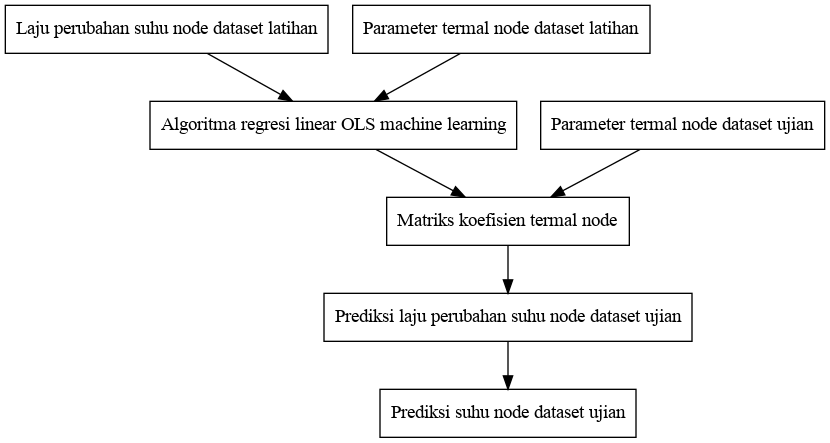
\includegraphics[width=0.8\textwidth]{fig/graph_mlsetup.png}
	\caption{Cara kerja model termal menggunakan metode \textit{machine learning}}
\label{fig:mlsetup}
\end{center}
\end{figure}

Dapat dilihat bahwa set latihan digunakan oleh algoritma \textit{machine
learning} untuk mempelajari hubungan antara parameter termal \textit{node}
dengan laju perubahan suhu \textit{node} per periode observasi dengan
menerapkan pendekatan regresi linear OLS seperti yang dijelaskan pada bagian
awal bab ini. Keluaran dari proses pelatihan ini adalah matriks yang berisi
koefisien persamaan termal satelit pada periode observasi.

Matriks koefisien tersebut kemudian diterapkan pada parameter-parameter
\textit{node} satelit set ujian sehingga menghasilkan prediksi laju perubahan
suhu \textit{node} satelit. Dari prediksi laju perubahan suhu \textit{node} dan
data waktu observasi satelit, prediksi suhu \textit{node} dapat dihitung.
Prediksi suhu \textit{node-node} satelit inilah yang akan dibandingkan dengan
suhu \textit{node-node} satelit dari data telemetri satelit dan akan
ditampilkan pada bagian Hasil Pemodelan Termal Satelit LAPAN-A3. Dengan
demikian, prediksi yang dihasilkan berasal dari model termal yang belum pernah
melihat set ujian sebelumnya karena model tersebut dilatih menggunakan set
latihan terpisah.

\section{Pelatihan dan Pengujian Model}

Dataset yang sudah disaring kemudian dibagi menjadi set latihan
(\textit{training}) dan ujian (\textit{test}) secara acak dengan menggunakan modul
Scikit-learn. Model \textit{machine learning} dilatih dan diuji untuk setiap
\textit{node} satelit per periode observasi. Pemodelan pada karya tulis ini
menggunakan rasio jumlah data pelatihan dibanding pengujian sebesar 0.7:0.3
serta pengaturan \textit{seed number} 0. Tabel \ref{table:dataset} memuat
detail jumlah dataset yang digunakan dalam pemodelan untuk kedua periode
observasi.

\begin{table}[!ht]
\begin{center}
\caption{Detail jumlah dataset model \textit{machine learning}}
\label{table:dataset}
\begin{tabular}{|c|cc|}
\hline
\multirow{2}{*}{Tanggal} & \multicolumn{2}{c|}{Dataset}                 \\ \cline{2-3} 
                         & \multicolumn{1}{c|}{Set latihan} & Set ujian \\ \hline
19 Mei 2018              & \multicolumn{1}{c|}{201}         & 87        \\ \hline
20 Mei 2018              & \multicolumn{1}{c|}{180}         & 78        \\ \hline
\end{tabular}
\end{center}
\vspace{-5mm}
\end{table}

Pelatihan dan pengujian model dipisah per tanggal observasi karena pada
Persamaan \ref{eq:lineq} koefisien $c_a$ mengandung nilai sudut bidang orbit
satelit terhadap Matahari $\beta$ yang dianggap konstan selama 1 periode
observasi. Nilai $\beta$ bergantung pada posisi Bumi relatif terhadap Matahari.
Dengan kata lain, nilai $\beta$ berubah seiring dengan pergantian hari
sepanjang tahun akibat revolusi Bumi mengitari Matahari \cite{m2019}.
